\chapter{Se servir des coordonnées}
{ }\hfill\textbf{Niveau:} débutant
\section{Présentation}
\noindent Dans ce chapitre, nous allons découvrir la primitive \texttt{fixeposition}. La zone de dessin est en fait muni d'un repère dont l'origine est située au centre de l'écran. On peut ainsi atteindre chacun des points de la zone de dessin à l'aide de ses coordonnées. \\ \\
\texttt{fpos liste}\hspace {4cm } \textcolor{red}{ \texttt{fpos [100 -250]}}\\
Déplace la tortue au point dont les coordonnées sont définis dans la liste.\\ \\
\\ Un petit exemple d'utilisation:\\ 
\texttt{ve fpos [200 100] fpos [50 -150] fpos [-100 -150]}
\begin{center}
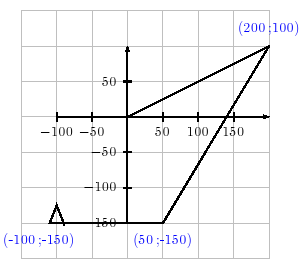
\includegraphics[scale=0.7]{images/fpos-coord.png}
\end{center}
\vspace{1cm}
\section{Exercice:}
\noindent
Réaliser cette figure en n'utilisant que les primitives: \texttt{fpos}, \texttt{ve}, \texttt{lc}, \texttt{bc}.\\
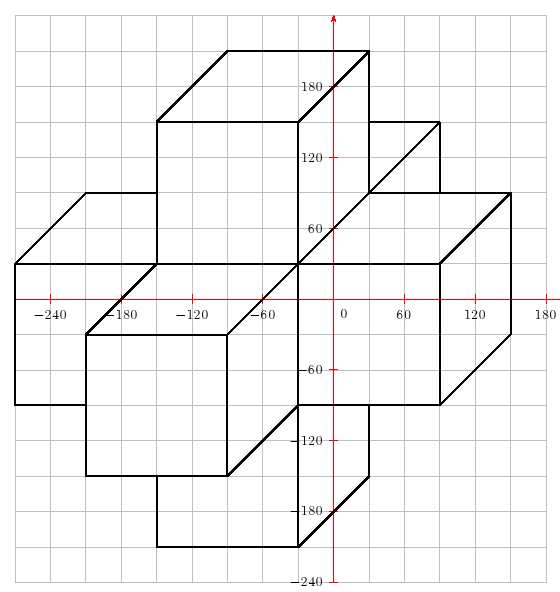
\includegraphics[scale=0.7]{images/fpos-cube.png}
